% These packages are optional, depending whether you want the features they provide.
% See the LaTeX Companion or other references for full information.
% !TEX TS-program = pdflatex
% !TEX encoding = UTF-8 Unicode

% This is a simple template for a LaTeX document using the "article" class.
% See "book", "report", "letter" for other types of document.

\documentclass[12pt]{article} % use larger type; default would be 10pt
\usepackage[T2A]{fontenc}
\usepackage[utf8]{inputenc} % set input encoding (not needed with XeLaTeX)
\usepackage[russian]{babel}
%%% Examples of Article customizations
% These packages are optional, depending whether you want the features they provide.
% See the LaTeX Companion or other references for full information.

%%% PAGE DIMENSIONS
\usepackage{geometry}

\usepackage{fancyhdr} 
\geometry{a4paper} % or letterpaper (US) or a5paper or....
% \geometry{margin=2in} % for example, change the margins to 2 inches all round
% \geometry{landscape} % set up the page for landscape
%   read geometry.pdf for detailed page layout information
\usepackage{sectsty}
\usepackage{graphicx} % support the \includegraphics command and options
\usepackage{mathtext}
\usepackage{amsmath}
\usepackage{amsfonts}
% \usepackage[indentfill]{indentskip} % Activate to begin indentagraphs with an empty line rather than an indent
\usepackage{biblatex}
\usepackage{hyperref}
\hypersetup{
  colorlinks=true,
  linkcolor=blue,
  urlcolor=green
}
%%% END Article customizations

%%% The "real" document content comes below...
\usepackage{setspace}
\usepackage[section]{minted}

%%% ToC (table of contents) APPEARANCE
\usepackage[nottoc,notlof,notlot]{tocbibind} % Put the bibliography in the ToC
\usepackage[titles,subfigure]{tocloft} % Alter the style of the Table of Contents

%\date{} % Activate to display a given date or no date (if empty),
         % otherwise the current date is printed 
\usepackage{physics}
\usepackage{float}
\begin{titlepage}
	\thispagestyle{empty}
	\begin{center}
	\large{МИНОБРНАУКИ РОССИИ}\\
	\footnotesize{ФЕДЕРАЛЬНОЕ ГОСУДАРСТВЕННОЕ БЮДЖЕТНОE ОБРАЗОВАТЕЛЬНОЕ УЧРЕЖДЕНИЕ}\\ 
	\footnotesize{ВЫСШЕГО ПРОФЕССИОНАЛЬНОГО ОБРАЗОВАНИЯ}\\ 
	\small{\textbf{«САНКТ-ПЕТЕРБУРГСКИЙ ГОСУДАРСТВЕННЫЙ ПОЛИТЕХНИЧЕСКИЙ УНИВЕРСИТЕТ ПЕТРА ВЕЛИКОГО»}}\\
	\hfill \break
	\normalsize{Институт компьютерных наук и технологий}\\
	\hfill \break
	\normalsize{Высшая школа искусственного интеллекта}\\
	\hfill\break
	\begin{center}
		\normalsize{Дисциплина: \\ПРОГРАММИРОВАНИЕ МИКРОКОНТРОЛЛЕРОВ}
	\end{center}
	\hfill \break
	\hfill \break
	\large{ОТЧЕТ}\\
	\large{По лабораторной работе №4}\\
	\medium{Тема: Таймер и Режим пониженного энергопотребления.}\\
	\hfill \break
	\hfill \break
	\hfill \break
	\hfill \break
	\hfill \break
	\hfill \break
\end{center}	

\normalsize{ 
	\begin{tabular}{ccc}
		Обучающийся &  гр. 3530201/10001 & Нгуен Куок Дат \\\\
		Руководитель & \hrulefill 				&Вербова Наталья Михайловна\\\\
	\end{tabular}
}\\
\hfill \break
\hfill \break
\hfill \break
\hfill \break
\begin{center} Санкт-Петербург 2022 
\end{center}
\end{titlepage}
\usepackage{indentfirst}

\begin{document}
\begin{center}
\input{titlepage}
\end{center}
\doublespacing
\tableofcontents
\newpage
\section{Цель и постановка задачи}
\subsection{Цель работы}
Ознакомится с основными методами формирования заданных интервалов времени и перевода микроконтроллера в режим пониженного энергопотребления. Закрепить навыки работы с осциллографом и оценочной платой MCBSTM32F200 в качестве измерительного генератора.
\subsection{Постановка задачи}

 Разработать программу для микроконтроллера (МК) STM32F200, которая:\\

\begin{itemize}
\item При помощи таймера
формирует периодическое попеременное включение и выключение светодиодов PG6 и PG7 с заданными временными характеристиками\\
\item При нажатии на кнопку
“WAKEUP” программа должна переводить МК в спящий режим, а при ее
отпускании пробуждать МК
\end{itemize}

\section{Выполнение задания}
\subsection{Направление светодиодов}
В этом задании использовал периферальный таймер \textbf{TIM2}, чтобы периодически генерировать прерывание, который определяет интервал последовательных включения и выключения светодиодов \textbf{PG7} и \textbf{PG8}. 

В каждом интервале включается в первой половине только \textbf{PG7} и в остальной половине только \textbf{PG8}. Чтобы его выполнить, включаем \textbf{PG7} если значение счетчика меньше половины максимум, а если не то, переключаем на \textbf{PG8}. 
\inputminted[firstline = 86, lastline = 95, breaklines]{C}{F:/git/micro/Lab4/Lab4.c}

\subsubsection*{Установка таймера \textbf{TIM2}}
Для установки таймера \textbf{TIM2} надо включить соответственное прерывание и конфигурировать \textbf{auto-reload value} и \textbf{prescaler}. Частота прерывания $f = \frac{f_\text{базовые часы}}{(TIMx\_PSC+1)(TIMx\_ARR+1)}$
Тогда чтобы прерывание вызывается каждые 2 секунды, может установить $TIM2\_PSC = 8400ul-1$ и $TIM2\_ARR = 1000ul-1$
\inputminted[firstline = 57, lastline = 69, breaklines]{C}{F:/git/micro/Lab4/Lab4.c}
\inputminted[firstline = 122, lastline = 124, breaklines]{C}{F:/git/micro/Lab4/Lab4.c}

\subsection{Установка прерывания}
Прерывание установляется на линии 0, которого вход \textbf{PA0}.

Во первых, надо дать МК знать, какой тип спящего режима будет. Здесь будет $low - power mode$.
\inputminted[firstline = 73, lastline = 76, breaklines]{C}{F:/git/micro/Lab4/Lab4.c}
Когда сообщаем МК чтобы спить, установить регистр $SCB_{SCR}$.\\

Алгорифм: Если МК не в спящем режиме, то установляем прерывание на режиме падания и переводить его в спящий режим; если МК уже в спящем режиме, то прерывание вызвано когда кнопка \textbf{PA0} отпускается, тогда пробуждаем МК и переводить прерывание на режиме спада. 

\inputminted[firstline = 103, lastline = 121, breaklines]{C}{F:/git/micro/Lab4/Lab4.c}



\section{Результат работы}
\subsection{Опыт A,B}
\begin{figure}[H]
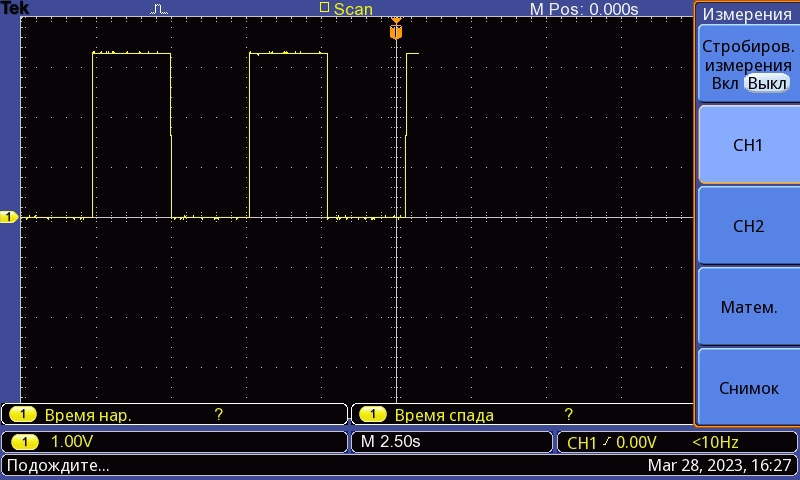
\includegraphics[width=0.9\textwidth]{exA.jpg}
\end{figure}

\begin{center}
Период = $250*2 = 500$ms\\
Частота = 1/период = 2Hz, совпадается с вычисленным значением. \\
$\text{T}_\text{вкл} = \text{T}_\text{выкл}  = 2.5$s\\
$\text{K}_\text{зап} = 50\%$
\end{center}

\subsection{Опыт C,D}
\begin{figure}[H]
	\begin{subfigure}
	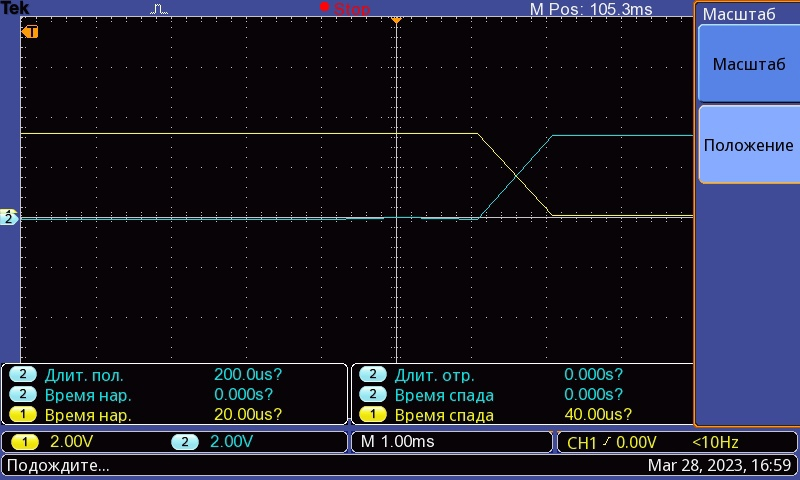
\includegraphics[width=0.4\textwidth]{exD1.jpg}
	\end{subfigure}
	\hfil
	\begin{subfigure}
	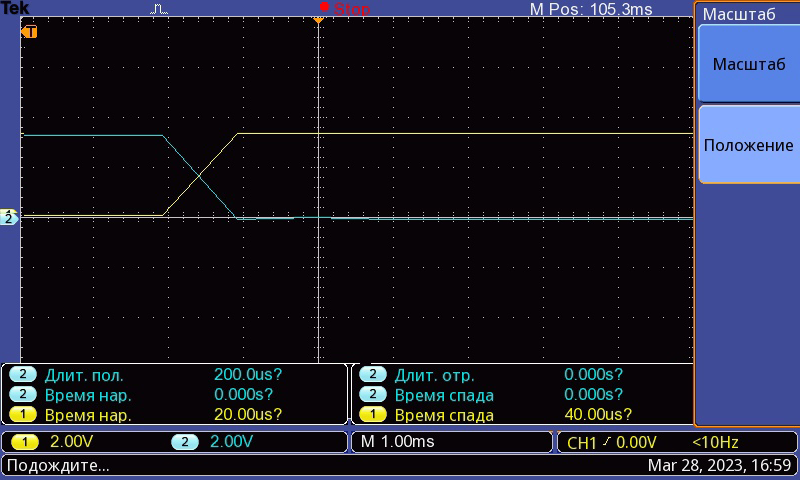
\includegraphics[width=0.4\textwidth]{exD2.png}
	\end{subfigure}
\end{figure}
\begin{center}
$\text{T}_\text{нар} = \text{T}_\text{спада}  = 1$ms\\
$\Phi = 90^\circ$\\
$\text{T}_\text{задержки} = 1$ms
\end{center}

\end{document}